% %%%%%%%%%%%%%%%%%%%%%%%%%%%%%%%%%%%%%%%%%%%%%%%%%%%%%%%%%%%%%%%%%%%%%%%%%%%%%
% %%%%%%%%%%%%%%%%%%%%%%%%%%%%%%%%%%%%%%%%%%%%%% Description of Numerical Model
% %%%%%%%%%%%%%%%%%%%%%%%%%%%%%%%%%%%%%%%%%%%%%%%%%%%%%%%%%%%%%%%%%%%%%%%%%%%%%

\chapter{Numerical Model}
\label{ch_model}

The model works in two and a half dimensions. A meridional slice of the magnetosphere is resolved. Fields are presumed to vary azimuthally according to a fixed modenumber \azm. Derivatives in $\phi$ are replaced by $i \azm$. Imaginary field values indicate a phase shift in the azimuthal direction. 


\todo{From Bob's 2013 paper\cite{lysak_2013} (which was also 2.5D): ``The shear \Alfven and compressional fast mode waves can be coupled not only by the Hall conductivity but also by inhomogeneities in the background plasma, which are unavoidable in a realistic magnetosphere [e.g., Lysak and Yoshikawa, 2006\cite{lysak_2006}; Waters et al., 2012\cite{waters_2013}]. This coupling requires a finite wave vector component in the azimuthal direction, i.e., a finite $m$ in the context of the present model. Because of the $\exp \arg{ i m \phi}$ dependence assumed in this model, the coupling from the inhomogeneity enters as an imaginary part of the coupled wave fields with respect to the initial fields, whereas the Hall conductivity appears in phase with the initial fields. Thus, although a fully three-dimensional model can give a more complete picture of wave propagation [e.g., Lysak, 2004\cite{lysak_2004}; Woodroffe and Lysak, 2012\cite{woodroffe_2012}], the present two-dimensional model serves to illustrate the nature of this coupling.''}

The use of a fixed modenumber allows a dramatic decrease in computational cost. Waves with very high azimuthal modenumber are prohibitively expensive to simulate since they can only be resolved if grid resolution is very fine in the azimuthal direction. 

\todo{Can we find a citation where someone explicitly talks about the computational cost of high-\azm simulations? Or is it just obvious Nyquist? }

This prevents the simultaneous consideration of dayside and nightside phenomena, but is fine for azimuthally-localized waves. As was shown by \cite{engebretson_1987}, and recently confirmed in detail by \cite{dai_2015}, Pc4 pulsations are generally confined to just a few hours MLT on the dayside. 

Driving with a compressional pulse from the outer boundary of a simulation is typical. This model also includes a novel driving mechanism: perturbations to the ring current. 

The code is linear. All magnetic fields are a first-order perturbation over the zeroth-order dipole field. This is a not-great assumption out towards the magnetopause. In practice, however, most activity is within $L \sim \SI{7}{\RE}$, where the dipole approximation is pretty good. 

Models with height-resolved ionospheres are a very recent development. Lysak presented his in 2013\cite{lysak_2013}. 

Ground signatures are fairly recent as well. 

\todo{Some ground signature work as far back as Greifinger and Greifinger in 1968\cite{greifinger_1968}, but there's been steady advancement. Lysak and Song, in 2006, were the first to work out ground signatures without the assumption of a single-frequency wave. }

\todo{The support software -- the driver and the plotter -- are significant too. Do they go in a section? In an appendix? }

\todo{Past FLR simulations focused on a single mode, didn't account well for the ionosphere, etc. Lee and Lysak 1989, 1990, 1991, Rankin et al 1993, 1995, 1999, Tikhonchuk and Rankin 2000, 2002. }

\todo{Past work that got ground signatures (without latitude-dependent zenith angle) Greifinger and Greifinger 1968, 1973, Hughes 1974, Sciffer and Waters 2002, Sciffer et al 2005. Better computation of ground signatures... Waters and Sciffer 2008, Sciffer and Waters 2011, Woodroffe and Lysak 2012. }

Note that the model uses megameters, seconds, megacoulombs, and grams as the fundamental units of length, time, charge, and mass respectively. As a result, electric field is measured in \si{\mV/\meter}, magnetic field is measured in \si{\nano\tesla}, and Poynting flux is measured in \si{\mW/\meter\squared}. The electric constant is expressed in \si{\milli\farad/\meter}, not in units of \ez, not that it really matters. 

% =============================================================================
% =============================================================================
% =============================================================================
\section{Coordinate System}
  \label{sec_coords}

When referring to fields in place, it's convenient to use lowercase\footnote{ Not to be confused with uppercase \X, \Y, and \Z, which orient relative to the sun; see \cref{ch_intro} } \x, \y, and \z in their usual dipolar sense. The unit vector \zhat is aligned with the dipole field (pointing outward in the northern hemisphere and inward in the southern hemisphere), while \xhat is perpendicular to \zhat within the meridional plane and \yhat points in the azimuthal direction. 

\todo{Double-check the signs for \x (radially inward or outward at the equator?) and \y (east or west?). }

\todo{Wait... are \x, \y, and \z the same as Radoski's coordinates? }

It's convenient to align the grid with the zeroth-order magnetic field, which is presumed to be a perfect dipole. Field line resonances (such as Pc4 pulsations) are guided by magnetic field lines. 

\todo{``ULF waves can be guided.'' Cite. }

A typical outermost field line has an equatorial radius of \SI{10}{\RE}. At this point, the ideal dipole approximation is suspect, particularly on the dayside. In practice, however, most wave activity is concentrated around $L \sim \num{7}$. 

Radoski did theoretical work in the following dipole coordinates\cite{radoski_1967_coords}. 
\begin{align}
  \label{radoski_coords}
  \radx & = -\frac{\sin^2 \theta}{r} & \rady & = \phi & \radz & = \frac{\cos \theta}{r^2}
\end{align}

\todo{The symbol $\nu$ is overused. Reserve it for collision frequency. Use something else here. }

It's also convenient to take into account the effects of the ionosphere, the lower boundary of which is governed by gravity, and thus has a more-or-less constant altitude. If the above coordinates are used, no line of constant $\radz$ coincides with the ionosphere, at least not over a significant range of latitudes. 

Many previous works have used an effective ionosphere of nonuniform altitude. 

\todo{Figure out which previous works are worth citing here. Options include Radoski 1967, Lee and Lysak 1989, 1991, Rankin et al 1993, 1994, Streltsov and Lotko 1995, 1999. }

\todo{``The ionosphere is important for \Alfven waves'' Cite? }

In order to accommodate dipole field lines as well as a fixed-altitude ionosphere, a nonorthogonal grid is necessary. Such a grid was worked out numerically by Proehl\cite{proehl_2002}, then formalized analytically by Lysak\cite{lysak_2004}:
\begin{align}
  \label{def_coords}
  \lysakx & = - \frac{R_I}{r} \sin^2 \theta & 
  \lysaky & = \phi &
  \lysakz & = \frac{R_I^2}{r^2} \frac{\cos \theta}{\cos \theta_0}
\end{align}

The term $R_I$ indicates the ionosphere's position relative to Earth's center. It's generally taken to be \SI{1}{\RE} + \SI{100}{\km}. 

Like \radx and \rady, the coordinates \lysakx and \lysaky index a field line. However, compared to \radz, \lysakz has been renormalized by $\cos \theta_0$, where $\theta_0$ is the colatitude where each field line intersects the ionosphere in the northern hemisphere. As a result, for all field lines, $\lysakz = \pm 1$ at the northern and southern foot points. 

In terms of the McIlwain parameter, $\lysakx = -\frac{R_I}{L}$, and $\cos \theta_0 = \sqrt{ 1 - \frac{R_I}{L} }$

Compared to \cref{radoski_coords}, \cref{def_coords} represents a renormalization of indexing along each field line. The field lines themselves are not deformed. 

\todo{Explain how we set up the grid. It should only take a paragraph or two -- it doesn't need its own section. }

\begin{figure}[H]
    \centering
    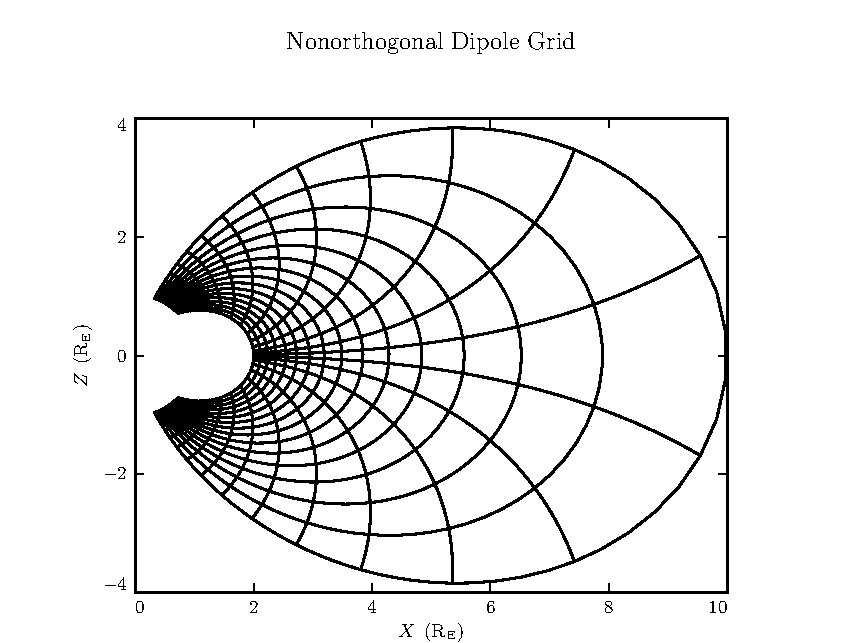
\includegraphics[width=\textwidth]{figures/grid.pdf}
    \caption[Nonorthogonal Dipole Grid]{
      The model's nonorthorthogonal dipole grid. Only every fifth point is shown in each direction. The grid resolution is highest near the ionosphere and lowest at large distances. The high concentration of grid points at the inner edge of the equator is a consequence of renormalizing the grid spacing with $\cos\theta_0$; whereas Radoski's dipole coordinates come to a singularity at the center of the Earth, Lysak's coordinates converge at the equatorial ionosphere. 
    }
    \label{fig_grid}
\end{figure}

% -----------------------------------------------------------------------------
% -----------------------------------------------------------------------------
% -----------------------------------------------------------------------------
\subsection{Covariant and Contravariant Bases}
  \label{sec_basis}

The coordinates defined in \cref{def_coords} are not orthonormal. As a result, it's necessary to consider covariant and contravariant basis vectors separately. 

Covariant basis vectors $\hat{e}_i \equiv \dd{\lysaki} \vec{x}$ are normal to the curve defined by constant $\lysaki$. 

Contravariant basis vectors $\hat{e}^i \equiv \dd{ \vec{x} } \lysaki$ are tangent to the coordinate curve. Equally, they're normal to the plane defined by constant $\lysakj$ for all $j \ne i$. 

The basis vectors are reciprocal to one another\cite{dhaeseleer_1991}, and can be used to define the metric tensor $g$. 
\begin{align}
  \label{metric_basics}
  \hat{e}^i \cdot \hat{e}_j &= \delta^i_j & \hat{e}_i \cdot \hat{e}_j &= g_{ij} & \hat{e}^i \cdot \hat{e}^j &= g^{ij}
\end{align}

Note $\delta^i_j$ is the Kronecker delta, $\varepsilon^{ijk}$ is the Levi-Civita symbol, and summation is implied over repeated indeces per Einstein's convention\cite{einstein_1916}. 

The metric tensor is used to map between the covariant and contravariant representations of a vector
\begin{align}
  \label{metric_usage}
  A_i &= g_{ij} A^j &
  & \text{and} &
  A^i &= g^{ij} A_j &
  & \text{where} &
  A_i &\equiv \vec{A} \cdot \hat{e}_i &
  & \text{and} &
  A^i &\equiv \vec{A} \cdot \hat{e}^i
\end{align}

The Jacobian, used for mapping differential volume elements between bases, can be expressed as the square root of the determinant of the metric tensor. 
\begin{align}
  \label{def_jacobian}
  \jac d\lysakx d\lysaky d\lysakz &= dV &
  & \text{where} &
  \jac &= \sqrt{ \varepsilon^{ijk} g_{1i} g_{2j} g_{3k} }
\end{align}

This quantity is also used when expressing a curl or cross product in generalized coordinates. 
\begin{align}
  \label{jacobian_usage}
  \lr{ \curl{A} }^i &= \frac{ \varepsilon^{ijk} }{\jac} \dd{\lysakj} A_k & \lr{ \cross{A}{B} }^i &= \frac{ \varepsilon^{ijk} }{\jac} A_j B_k
\end{align}

% -----------------------------------------------------------------------------
% -----------------------------------------------------------------------------
% -----------------------------------------------------------------------------
\subsection{Mapping to Physical Coordinates}

The full expression for the basis vectors, metric tensor, and Jacobian determinant discussed in \cref{sec_basis} can be found in the appendix of \cite{lysak_2004}. 

\todo{These expressions should probably be written out an in appendix here too...}

The basis vectors can be renormalized to produce unit vectors along the dipole coordinates \x, \y, and \z. 
\begin{align}
  \label{def_xyz_directions}
  \xhat &= \frac{1}{ \sqrt{ g^{11} } } \hat{e}^1 &
  \yhat &= \frac{1}{ \sqrt{ g^{22} } } \hat{e}^2 &
  \zhat &= \frac{1}{ \sqrt{ g_{33} } } \hat{e}_3
\end{align}

In addition, this coordinate system provides horizontal and radial unit vectors. Note that \cref{def_rqf_directions} is valid only at the ionospheric boundary. 
\begin{align}
  \label{def_rqf_directions}
  \qhat &= \frac{1}{ \sqrt{ g_{11} } } \hat{e}_1 &
  \fhat &= \frac{1}{ \sqrt{ g_{22} } } \hat{e}_2 &
  \rhat &= \frac{1}{ \sqrt{ g^{33} } } \hat{e}^3
\end{align}

% =============================================================================
% =============================================================================
% =============================================================================
\section{Ionospheric Profile}
  \label{sec_ionos}

The ionospheric profiles used in this model are based on values tabulated in the Appendix B of Kelley's book\cite{kelley_1989}. They were adapted by Lysak\cite{lysak_2013} to take into account the effect of the magnetosphere's latitude-dependent density profile. 

Mean molecular mass of \SI{28}{\amu} at \SI{100}{\km}, \SI{16}{\amu} around \SI{400}{\km}, down to \SI{1}{\amu} above \SI{1400}{\km}. 

Simulations are carried out using four profiles: active day, quiet day, active night, quiet night. 

Profiles are static for the duration of a simulation. Even so-called ultra low frequency waves are still much faster than convective timescales. 

\todo{Come up with a characteristic convective timescale or two, and cite it. }

% -----------------------------------------------------------------------------
% -----------------------------------------------------------------------------
% -----------------------------------------------------------------------------
\subsection{Conductivity}

The effects of mean molecular mass on conductivity are computed per the usual definitions. 
\begin{align}
  \sp &= \displaystyle\sum_s \frac{n_s q_s^2}{m_s} \frac{\nu_s}{\nu_s^2 + \Omega_s^2} &
  \sh &= -\displaystyle\sum_s \frac{n_s q_s^2}{m_s} \frac{\Omega_s}{\nu_s^2 + \Omega_s^2} &
  \sz &= \displaystyle\sum_s \frac{n_s q_s^2}{m_s \nu_s}
\end{align}

Each profile is resolved to an altitude of about $\SI{e4}{\km}$, and include well-resolved $E$, $F_1$, and $F_2$ layers. 

\todo{Talk about the ionospheric layers, probably in the introduction. }

\begin{figure}[H]
    \centering
    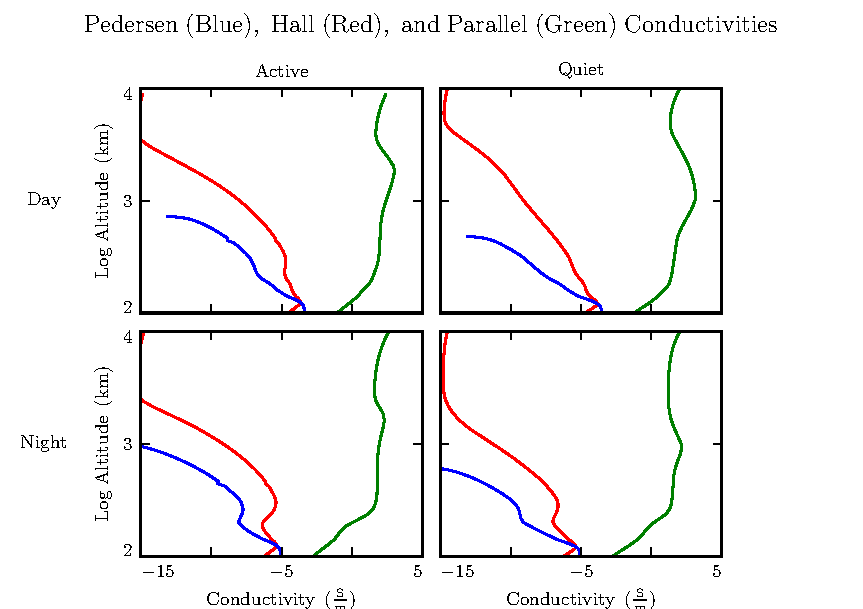
\includegraphics[width=\textwidth]{figures/sigma.pdf}
    \caption[Ionospheric Conductivity Profiles]{
      Ionospheric conductivity profiles, adapted by Lysak\cite{lysak_2013} from Appendix B of Kelley's textbook\cite{kelley_1989}. 
    }
    \label{fig_sigma}
\end{figure}

\todo{What is the height-interated conductivity for each profile? }

% -----------------------------------------------------------------------------
% -----------------------------------------------------------------------------
% -----------------------------------------------------------------------------
\subsection{\Alfven Speed}

The \Alfven speed is computed from Kelley's low-density profile, modified to take into account the local density. The density, in turn, is the sum of a plasmaspheric profile and a high-latitude auroral profile. 
\begin{align}
  \ep &= \text{(low-density tabulated value)} + \frac{ n \bar{m} }{B_0^2}
\end{align}

\todo{What's a clean way of showing the low-density \ep that we read in? }

\todo{Does Kelley list the electric constant or the \Alfven speed? }

Where $\bar{m}$ is the ambient mean molecular mass and $B_0$ is the zeroth-order magnetic field strength, $B_0 = \SI{3.11e4}{\nano\tesla} \lr{ \frac{R_E}{r} }^3 \sqrt{ 1 + 3 \cos^2 \theta }$. Note that \SI{3.11e4}{\nano\tesla} is the value of the Earth's magnetic field at the equator on Earth's surface. 

\todo{Cite this number? }

\begin{figure}[H]
    \centering
    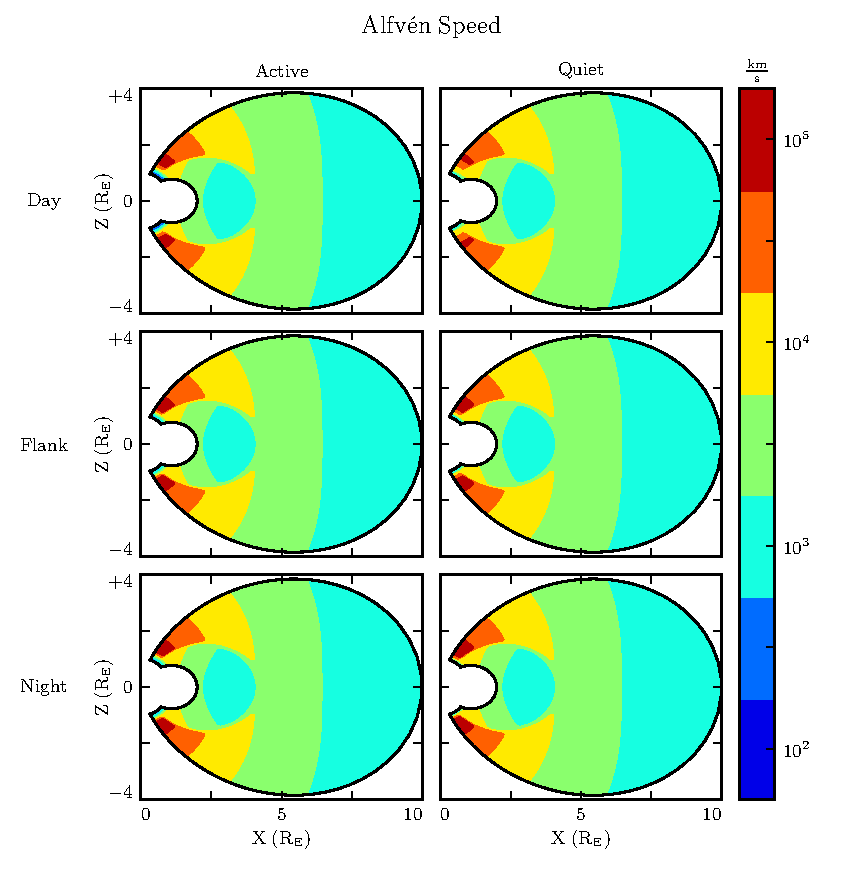
\includegraphics[width=\textwidth]{figures/va.pdf}
    \caption[\Alfven Speed Profiles]{
      \Alfven speed profiles, adapted by Lysak\cite{lysak_2013} from Appendix B of Kelley's textbook\cite{kelley_1989}. 
    }
    \label{fig_va}
\end{figure}

\todo{Above the profile, Bob scales the value that's read in as $r^5$ or something. Is there a citation for that? }

The \Alfven speed is then computed per $\va^2 \equiv \frac{1}{\mz \ep}$. 

\begin{figure}[H]
    \centering
    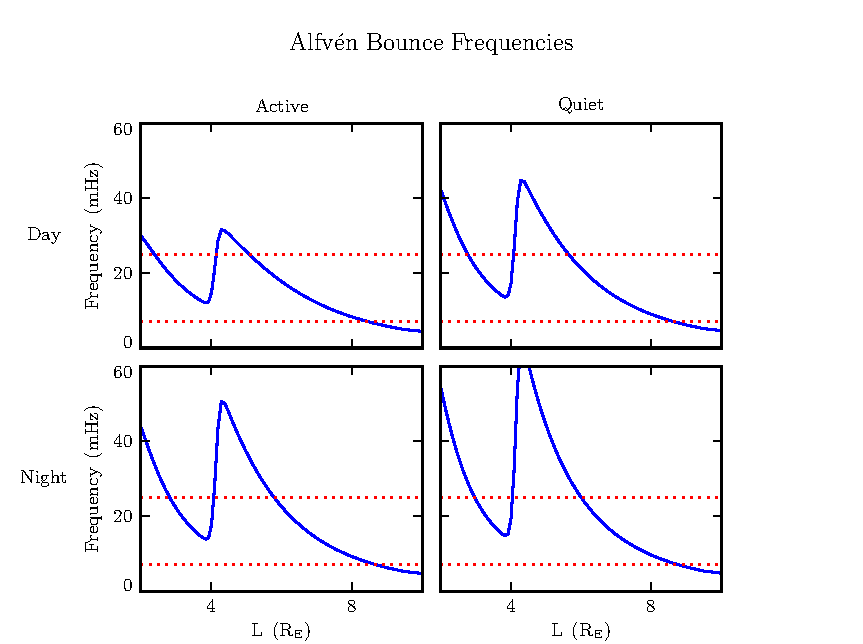
\includegraphics[width=\textwidth]{figures/fa.pdf}
    \caption[\Alfven Bounce Frequency Profiles]{
      \Alfven bounce frequency profiles, computed by integrating the the \Alfven speed back and forth over a field line. $f_A = \lrb{ \oint \frac{dz}{v_A} }^{-1}$. Dotted lines indicate the Pc4 frequency range, \SIrange{7}{25}{\mHz}. In each profile, the effect of the plasmapause is clearly visible, centered at $L=4$. Field lines just inside and just outside the plasmapause appear susceptible to resonance in the Pc4 band. 
    }
    \label{fig_fa}
\end{figure}

\todo{Talk about how the size of the plasmasphere can be adjusted, and \SI{4}{\RE} is just a typical value. }

\todo{Explain how the \Alfven speed constrains the time step. }

% =============================================================================
% =============================================================================
% =============================================================================
\section{Maxwell's Equations}
  \label{sec_eqns}

The model simulates the evolution of electric and magnetic fields in accordance with Maxwell's equations. Specifically, magnetic fields are advanced using \farlaw, and electric fields with \amplaw. Kirchhoff's formulation of \ohmlaw ($\vec{J} = \tensor{\sigma} \cdot \vec{E}$) is used to eliminate the explicit current dependence in \amplaw. 
\begin{align}
  \label{def_eqns}
  \ddt \vec{B} &= - \curl{E} &
  \tensor{\epsilon} \cdot \ddt \vec{E} &= \frac{1}{\mu_0} \curl{B} - \tensor{\sigma} \cdot \vec{E}
\end{align}

% -----------------------------------------------------------------------------
% -----------------------------------------------------------------------------
% -----------------------------------------------------------------------------
\subsection{Notation and Optimization}

Algebra is carried out on paper, producing expressions where each field value is a linear combination of previous field values. These coefficients are computed before the main loop begins. This offers a significant reduction in floating point operations each iteration. 

The \assign operator is used to indicate assignment, rather than equality. Values on the left are new, and those on the right are old. New and old magnetic field values are offset by \dt; electric field values staggered by $\frac{\dt}{2}$. As an example of this notation, \cref{def_assign} integrates \farlaw over a time step, assuming that the curl of the electric field varies slowly compared to \dt: 
\begin{align}
  \label{def_assign}
  \begin{split}
  \int_0^{\dt} \! dt \, \ddt \vec{B} &= - \displaystyle\int_0^{\dt} \! dt \, \curl{E} \\ 
  \left. \vec{B} \right|_{\dt} - \left. \vec{B} \right|_0 &= \left. - \dt \, \curl{E} \right|_{ \frac{\dt}{2} } \\
  \vec{B} &\assign \vec{B} - \dt \, \curl{E}
  \end{split}
\end{align}

It's also beneficial to store the curl of each field, rather than take derivatives on the fly. The following sections make use of the shorthand $\vec{C} \equiv \curl{E}$ and $\vec{F} \equiv \curl{B}$. Or, recalling \cref{jacobian_usage}, 
\begin{align}
  \label{def_curls}
  C^i & = \frac{ \varepsilon^{ijk} }{\jac} \dd{\lysakj} E_k &
  F^i & = \frac{ \varepsilon^{ijk} }{\jac} \dd{\lysakj} B_k
\end{align}

Only covariant field components are stored. Only contravariant curl components are stored. This cuts down on memory use, while also eliminating the time spent rotating between bases; rotations between covariant and contravariant bases are built into the precomputed coefficients. 

% -----------------------------------------------------------------------------
% -----------------------------------------------------------------------------
% -----------------------------------------------------------------------------
\subsection{Magnetic Fields}

Taking advantage of the shorthand defined in \cref{def_curls}, \farlaw is simply written
\begin{align}
  \label{farlaw_ijk}
  \ddt B^i &= - C^i
\end{align}

Or, using the metric tensor to cast the magnetic field in terms of its covariant components, and writing out each coefficient explicitly,
\begin{align}
  \begin{split}
  B_1 &\assign B_1 - g_{11} \, \dt \, C^1 - g_{13} \, \dt \, C^3 \\
  B_2 &\assign B_2 - g_{22} \, \dt \, C^2 \\
  B_3 &\assign B_3 - g_{31} \, \dt \, C^1 - g_{33} \, \dt \, C^3
  \end{split}
\end{align}


% -----------------------------------------------------------------------------
% -----------------------------------------------------------------------------
% -----------------------------------------------------------------------------
\subsection{Electric Fields}
  \label{sec_e}

\amplaw, can be solved with integrating factors. From \cref{def_eqns}, 
\begin{align}
  \tensor{\epsilon} \cdot \ddt \vec{E} &= \frac{1}{\mu_0} \curl{B} - \tensor{\sigma} \cdot \vec{E}
\end{align}

The permittivity tensor can be trivially inverted. 
\begin{align}
  \label{amp_tensor}
  \lr{ \tensor{\Omega} + \tensor{ \mathbb{I} } \ddt } \cdot \vec{E} &= \tensor{v}^2 \cdot \vec{F}
\end{align}

Where $\tensor{ \mathbb{I} }$ is the identity tensor and in \x-\y-\z coordinates, 
\begin{align}
  \tensor{v}^2 &\equiv \frac{1}{\mz} \tensor{\epsilon}^{-1} = 
    \mmm{\va^2}{0}{0}
        {0}{\va^2}{0}
        {0}{0}{c^2}
  && \text{and} &
  \tensor{\Omega} &\equiv \tensor{\epsilon}^{-1} \cdot \tensor{\sigma} = 
    \mmm{ \frac{\sp}{\ep} }{ -\frac{\sh}{\ep} }{0}
        { \frac{\sh}{\ep} }{ \frac{\sp}{\ep} }{0}
        {0}{0}{ \frac{\sz}{\ez} } 
\end{align}

Using integrating factors, \cref{amp_tensor} gives
\begin{align}
  \vec{E} &\assign \exp \arg{ -\tensor{\Omega} \; \dt } \cdot \vec{E} + \dt \, \tensor{v}^2 \cdot \exp \arg{ -\tensor{\Omega} \; \tfrac{\dt}{2} } \cdot \vec{F}
\end{align}

\todo{Do we need to be careful here about the difference between a matrix and a tensor? }

The tensor exponential can be evaluated by considering the diagonal and off-diagonal terms separately. 
\begin{align}
  \tensor{\Omega} &= \tensor{\Omega}'
    + \frac{\sh}{\ep} 
    \mmm{0}{-1}{0}
        {1}{0}{0}
        {0}{0}{0} && \text{where} &
  \tensor{\Omega}' &=
    \mmm{ \frac{\sp}{\ep} }{0}{0}
        {0}{ \frac{\sp}{\ep} }{0}
        {0}{0}{ \frac{\sz}{\ez} }
\end{align}

Note that tensors are remarkably well-behaved when exponentiated\cite{hall_2015}. Because $\tensor{\Omega}'$ is diagonal, and thus the two commute,  
\begin{align}
  \exp \arg{ \tensor{T} } &= \displaystyle\sum_n \frac{1}{ n! } \tensor{T}^n &
  & \text{and} &
  \exp \arg{ \tensor{T} + \tensor{T}' } &= \exp \arg{ \tensor{T} } \exp \arg{ \tensor{T}' }
\end{align}

The off-diagonal terms collapse into sines and cosines, indicating a rotation about \z. 
\begin{align}
  \label{amp_final}
  \vec{E} &\assign \exp \arg{ -\tensor{\Omega}' \; \dt } \cdot \tensor{R}_z \arg{ \tfrac{-\sh \dt}{\ep} } \cdot \vec{E}
   + \dt \, \tensor{v}^2 \cdot \exp \arg{ -\tensor{\Omega}' \; \tfrac{\dt}{2} } \cdot \tensor{R}_z \arg{ \tfrac{-\sh \dt}{2 \ep} } \cdot \vec{F}
\end{align}

Where 
\begin{align}
  \tensor{R}_z \arg{\theta} &= 
  \mmm{\cos\theta}{-\sin\theta}{0}
      {\sin\theta}{\cos\theta}{0}
      {0}{0}{1}
\end{align}

The parallel term of term of \cref{amp_final} is simply
\begin{align}
  E_\parallel \assign E_\parallel \exp \arg{ \tfrac{- \sz \dt}{\ez} } + c^2 \dt F_\parallel \exp \arg{ \tfrac{- \sz \dt}{2 \ez} }
\end{align}

Or, in covariant terms, 
\begin{align}
  \label{amp_para}
  E_3 \assign E_3 \exp \arg{ \tfrac{- \sz \dt}{\ez} } + c^2 \dt \lr{ g_{31} F^1 + g_{33} F^3 } \exp \arg{ \tfrac{- \sz \dt}{2 \ez} }
\end{align}

For the ionospheric profiles and time steps employed by this model, $\frac{\sz \dt}{\ez}$ is never smaller than $10^3$. As a result, $\exp \arg{ \frac{- \sz \dt}{\ez} }$ is far too small to be stored in a double precision variable. That is, this simulation takes $E_\parallel$ (and, as a result, $E_3$) to be uniformly zero. 

This, obviously, precludes any discussion of parallel electric fields or parallel currents. These topics are revisited in \cref{ch_inertia}. 

Not unrelatedly, recalling the definition of the plasma frequency and parallel conductivity from \cref{def_basics}, $\frac{\sz}{\ez}$ can also be written $\frac{\op^2}{\nu}$. 

The plasma frequency is very fast. 

The perpendicular components of \cref{amp_final}, mapped from the physical basis to the contravariant basis (per \cref{def_xyz_directions}) to the covariant basis (per \cref{metric_usage}), give
\begin{alignat}{6}
  \label{e1_final}
  & E_1 + \frac{ g^{13} }{ g^{11} } && E_3 \assign &&   && E_1 && \cos \arg{ \tfrac{- \sh \dt}{\ep} } \exp \arg{ \tfrac{- \sp \dt}{\ep} } &&  \notag \\
  &                                 &&             && + && E_2 && \sin \arg{ \tfrac{- \sh \dt}{\ep} } \exp \arg{ \tfrac{- \sp \dt}{\ep} } &&  \sqrt{ \frac{ g^{22} }{ g^{11} } } \notag \\
  &                                 &&             && + && E_3 && \cos \arg{ \tfrac{- \sh \dt}{\ep} } \exp \arg{ \tfrac{- \sp \dt}{\ep} } &&  \frac{ g^{13} }{ g^{11} } \\
  &                                 &&             && + && F^1 && \cos \arg{ \tfrac{- \sh \dt}{2\ep} } \exp \arg{ \tfrac{- \sp \dt}{2\ep} } &&  \frac{\va^2 \dt}{ g^{11} } \notag \\
  &                                 &&             && + && F^2 && \sin \arg{ \tfrac{- \sh \dt}{2\ep} } \exp \arg{ \tfrac{- \sp \dt}{2\ep} } &&  \frac{\va^2 \dt}{ \sqrt{ g^{11} g^{22} } } \notag \\
  \intertext{and}
  \label{e2_final}
  & && E_2 \assign && - && E_1 && \sin \arg{ \tfrac{- \sh \dt}{\ep} } \exp \arg{ \tfrac{- \sp \dt}{\ep} } &&  \sqrt{ \frac{ g^{11} }{ g^{22} } } \notag \\
  & &&             && + && E_2 && \cos \arg{ \tfrac{- \sh \dt}{\ep} } \exp \arg{ \tfrac{- \sp \dt}{\ep} } &&  \notag \\
  & &&             && - && E_3 && \sin \arg{ \tfrac{- \sh \dt}{\ep} } \exp \arg{ \tfrac{- \sp \dt}{\ep} } &&  \frac{ g^{13} }{ \sqrt{ g^{11} g^{22} } } \\
  & &&             && - && F^1 && \sin \arg{ \tfrac{- \sh \dt}{2\ep} } \exp \arg{ \tfrac{- \sp \dt}{2\ep} } &&  \frac{\va^2 \dt}{ \sqrt{ g^{11} g^{22} } } \notag \\
  & &&             && + && F^2 && \cos \arg{ \tfrac{- \sh \dt}{2\ep} } \exp \arg{ \tfrac{- \sp \dt}{2\ep} } &&  \frac{\va^2 \dt}{ g^{22} } \notag
\end{alignat}

The $E_3$ terms can be ignored at present, but \cref{ch_inertia} references back to them. 

% =============================================================================
% =============================================================================
% =============================================================================
\section{Driving}
  \label{sec_driving}

If no energy is added, the simulation is pretty boring. Everything just stays zero. 

% -----------------------------------------------------------------------------
% -----------------------------------------------------------------------------
% -----------------------------------------------------------------------------
\subsection{Outer Boundary Compression}

Driving from the outer boundary is the traditional way to do it. 

\todo{Cite and briefly explain past work done with compressional driving. }

As discussed in \cref{sec_math_implications}, \Alfven waves become guided when the azimuthal modenumber is large. The energy all stays close to the outer boundary. No field line resonances of significant strength are created within the magnetosphere. 

\todo{Should the model be presented first, or the dispersion relation? It's natural to talk about the ionospheric profiles when presenting the model, which the dispersion relation relies upon. But it's convenient, here, to be able to talk about how \Alfven waves become guided at large \azm. That probably means that the math should go first, and the ionospheric profiles should be squeezed in somewhere earlier. }

\begin{figure}[H]
    \centering
    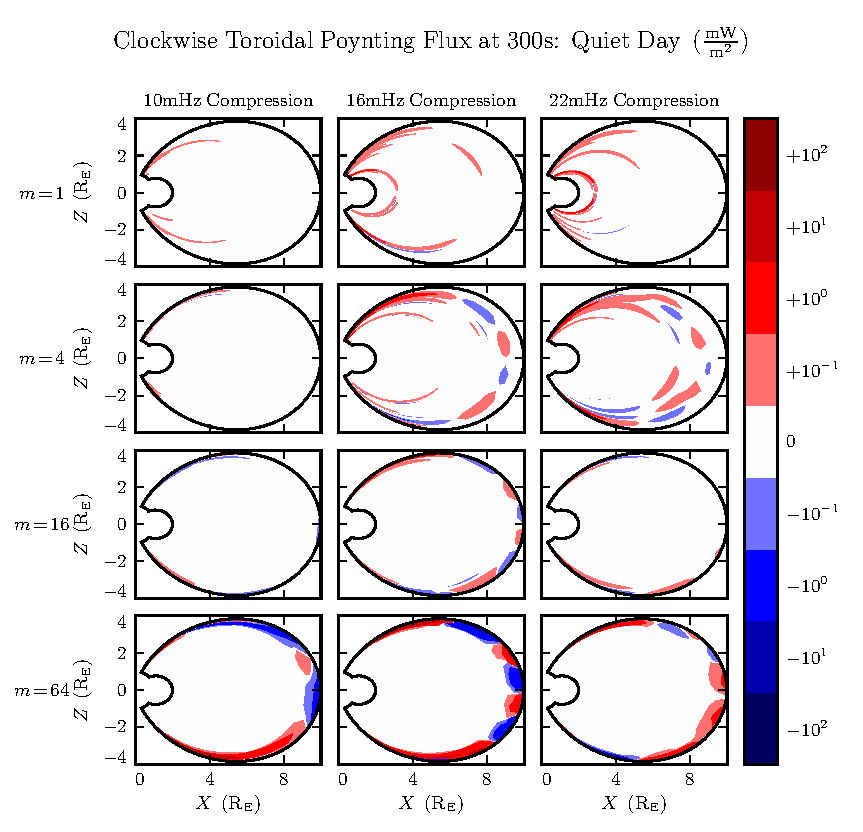
\includegraphics[width=\textwidth]{figures/Stor_B_2.pdf}
    \caption[Decreasing Penetration with Increasing Modenumber]{
      When the azimuthal modenumber is small, energy delivered through compression of the outer boundary is able to propagate across field lines and stimulate field line resonances in the inner magnetosphere. However, as modenumber increases, \Alfven waves become increasingly guided. As a result, energy delivered at the outer boundary cannot penetrate to the inner magnetosphere. Note that the large values on the bottom row should be taken with a grain of salt; it's not clear that the simulation is reliable when waves are continuously forced against the boundary. 
    }
    \label{fig_Stor_B_2}
\end{figure}

Compressional driving is applied by setting the value of $B_3$ at the outer boundary. 

A compression might reasonably be expected to drive waves with long azimuthal wavelengths. However, there is some indication that waves with short azimuthal wavelength can be driven as well, such as through Kelvin-Helmholtz interactions. 

\todo{Find this claim again and cite it. }

% -----------------------------------------------------------------------------
% -----------------------------------------------------------------------------
% -----------------------------------------------------------------------------
\subsection{Ring Current Modulation}

Pc4 pulsations with high azimuthal modenumber are known to be driven from within the magnetosphere, such as through drift-resonant interactions with energetic radiation belt and ring current particles. 

\todo{Cite. }

Substorm injection can cause localized ring current behavior. 

\todo{UNH was looking at this at AGU. Check if they have published yet. }

During geomagnetically active times, the ring current is a dynamic region. It's easy to imagine localized perturbations. 

It's difficult to estimate how large such perturbations might be. The following is a kludgey estimate. 

\begin{figure}[H]
    \centering
    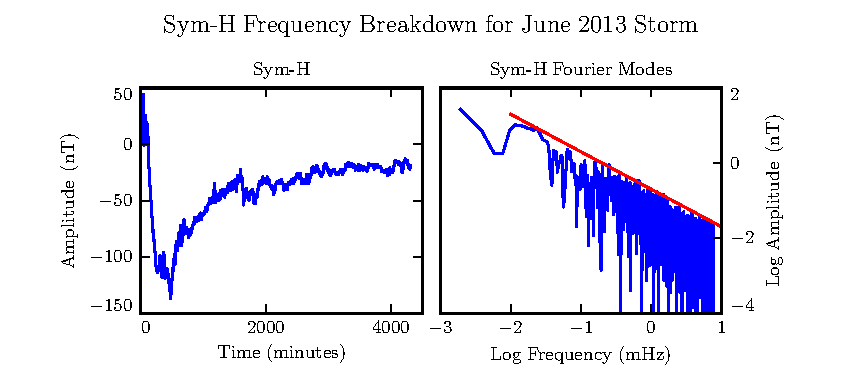
\includegraphics[width=\textwidth]{figures/symh.pdf}
    \caption[Sym-H Fourier Components for June 2013 Storm ]{
      The Sym-H storm index (from NASA CDAWeb\cite{nasa_cdaweb}) measures magnetic perturbations on Earth's surface due to ring current activity. It is measured once per minute, so Fourier amplitudes in the Pc4 range cannot be measured directly. However, they can be inferred by fitting the pink noise. The red line shows a fit to the top of the distribution, $\sim$ \SI{e-2}{\nano\tesla} $\lr{ \frac{ \SI{20}{\mHz} }{f} }$. 
    }
    \label{fig_symh}
\end{figure}

Sym-H is like Dst, but with greater time resolution. 

The noise suggests that a Fourier component with a period of about \SI{1}{\minute} could have an amplitude around \SI{e-2}{\nano\tesla}. 

If the driving is delivered at $L=5$, with a standard deviation of \SI{0.5}{\RE} in the radial direction and \SI{5}{\degree} angularly, that corresponds to a current density on the order of \SI{e-4}{\uA/\meter\squared}. This comes from approximating the ring current as a ring of current. Of course, Sym-H is measured at Earth's surface, not at the center of the ring; this gives a geometric factor of about two. 

\todo{What electric field magnitude does this correspond to? }

Current driving is applied by adding an additional current term. \amplaw becomes
\begin{align}
  \tensor{\epsilon} \cdot \ddt \vec{E} &= \frac{1}{\mu_0} \curl{B} - \tensor{\sigma} \cdot \vec{E} - \vec{J}_{drive}
\end{align}

And this driving term is absorbed into the curl by revising \cref{def_curls} from $\vec{F} \equiv \curl{B}$ to $\vec{F} \equiv \curl{B} - \vec{J}_{drive}$. (As a result, \cref{e1_final,e2_final} do not change.)

Notably, Sym-H is a global quantity; it's not ideally suited for making estimates of localized inhomogeneity. 

Furthermore, Sym-H has a time resolution of \SI{1}{\minute}. It can hardly be said to carry information about oscillations at frequencies of less than two minutes. 

Sym-H gives no way to estimate azimuthal modenumber. That's based on Pc4 observations. Dai\cite{dai_2015} observed modenumbers approaching \num{100}. 

A kludgey estimate is better than no estimate. 

% =============================================================================
% =============================================================================
% =============================================================================
\section{Boundary Conditions}
  \label{sec_bcs}

The grid can't go on forever. There have to be special cases at the edges. 


% -----------------------------------------------------------------------------
% -----------------------------------------------------------------------------
% -----------------------------------------------------------------------------
\subsection{Parity and Interpolation}

Computation takes place on a staggered grid. 

Field values are offset to ensure that most differences are centered. For example, $\ddt B_2$ depends on $\dd{\lysakx} E_3$ and $\dd{\lysakz} E_1$. If $B_2$ is defined at even $i$, $E_3$ is defined at odd $i$, so that $B_2$ is defined on the same grid points as $\frac{ E_3 \lrb{i+1} - E_3 \lrb{i-1} }{ \lysakx \lrb{i+1} - \lysakx \lrb{i-1} }$. 

\todo{Make sure the example uses the currect parities. }

\todo{Find a citation for the wigglies that occur if field values are defined on all grid points, due to the weak coupling. This problem is apparently well-known. }

Values are sometimes needed off-parity. $E_1$ and $E_2$ are not defined at the same grid locations, but they are coupled directly by the Hall conductivity. And $B_1$ and $B_3$ are coupled by the non-orthogonality of the grid. When off-parity values are needed, they are interpolated from their neighbors. 

Differentiation and interpolation are good to second order on the nonuniform grid. Like the coefficients for Maxwell's equations, differentiation and interpolation weights are computed during setup to save time during iteration. 

Electric fields go to zero at the innermost and outermost field lines (Dirichlet boundary conditions). Magnetic fields have zero derivative (Neumann boundary conditions). For components not defined at the exact boundary, these rules are applied when differentiating or interpolating; they set the effective value just outside the grid. 

These boundary conditions can in principle cause nonphysical reflection at the boundary. In practice, that is not an issue. Wave activity is concentrated well away from the boundaries. In fact, reversing the Dirichlet and Neumann boundary conditions has little effect. 

(Of course, an inconsistent boundary condition -- like using the same boundary condition for a field and its derivative -- causes instability.)

% -----------------------------------------------------------------------------
% -----------------------------------------------------------------------------
% -----------------------------------------------------------------------------
\subsection{Coupling to the Atmosphere}

Conditions at the ionospheric boundaries are set by coupling to the atmosphere. This also allows the computation of ground fields. 

It's reasonable to approximate the atmosphere as a perfect insulator, giving $\curl{B}=0$. Combining with $\div{B}=0$ per Maxwell's equations, ensures the existence of a scalar magnetic potential $\Psi$ such that $\vec{B}=\grad{\Psi}$ and $\Psi$ satisfies Laplace's equation, $\nabla^2 \Psi = 0$. 

Laplace's equation can be solved analytically; in spherical coordinates, the solutions are spherical harmonics. However, a numerical solution is preferrable to ensure orthonormality on a discrete (and incomplete -- there are no grid points at the poles or equator) grid. After separating out the radial and azimuthal dependence in the usual way, the latitudinal component of Laplace's equation (in terms of $s \equiv - \sin^2 \theta$) is
\begin{align}
  \label{laplace}
  \lr{ 4 s^2 + 4s } \frac{d^2}{ds^2} Y_\ell + \lr{ 4 + 6 s } \frac{d}{ds} Y_\ell - \frac{\azm^2}{s} Y_\ell &= \ell \lr{ \ell + 1 } Y_\ell
\end{align}

Using centered differences to express the derivatives, \cref{laplace} is a system of linear equations, one per field line. It can be solved numerically for eigenvalues $\ell \lr{\ell + 1}$ and eigenvectors (harmonics) $Y_\ell$. In terms of those harmonics, and noting that the model uses a fixed azimuthal modenumber \azm, $\Psi$ between $R_E$ and $R_I$ can be expressed
\begin{align}
  \label{psi_expansion}
  \Psi \arg{r, \theta, \phi} &= \displaystyle\sum_\ell \lr{ \alpha_\ell \, r^\ell + \beta_\ell \, r^{-\ell - 1} } Y_\ell \arg{\theta} \exp \arg{i \azm \phi}
\end{align}

As a boundary condition for $\Psi$, Earth's crust is assumed to be a perfect conductor, forcing the magnetic field at the boundary to be perfectly horizontal. That is, $B_r = \dd{r} \Psi = 0$. Then, noting that the harmonics $Y_\ell$ are orthonormal (so each term of the sum must be zero), 
\begin{align}
  \label{beta_solution}
  \beta_\ell &= \frac{\ell}{\ell + 1} R_E^{2 \ell + 1} \alpha_\ell
\end{align}

Note that the explicit $\phi$ dependence has been dropped. The entire simulation shares a fixed modenumber, so it's sufficient to find $\Psi$ at $\phi=0$. 

At the top of the atmosphere, the radial magnetic field is again used as a boundary condition, this time to compute the weights $\alpha_\ell$. 

\todo{Something something thin horizontal current sheet at $R_I$. }

Taking the shorthand $\lambda_I \equiv \frac{R_E}{R_I} \sim \num{0.975}$
\begin{align}
  B_r &= \displaystyle\sum_\ell \ell \, \alpha_\ell \, R_I^{\ell-1} \, \lr{ 1 - \lambda_I^{2 \ell - 1} } Y_\ell
\end{align}

\todo{Settle on good notation for taking the inner product of harmonics. It's a vector in the sense that it's a one-dimensional array of values, but not in the physical sense. Indexing -- $B_r\lrb{i}$ -- also seems awkward. }

The sum can be collapsed by ``integrating" over a harmonic. The inverse harmonics are obtained by inverting the eigenvector matrix. Then $Y_\ell \cdot Y_{\ell'}^{-1} = \delta_{\ell \ell'}$ by construction. 
\begin{align}
  \label{alpha_solution}
  \alpha_\ell &= \frac{ 1 }{\ell \, R_I^{\ell-1} } \frac{ B_r \cdot Y_\ell^{-1} }{ 1 + \lambda_I^{2 \ell + 1} }
\end{align}

Combining \cref{psi_expansion,beta_solution,alpha_solution} allows the expression of $\Psi$ at the top and bottom of the atmosphere as a linear function of the radial magnetic field at the boundary. 
\begin{align}
  \label{psi_final}
  \begin{split}
  \Psi_E &= \displaystyle\sum_\ell Y_\ell \; \frac{R_I}{\ell} \frac{ \frac{2 \ell - 1}{\ell - 1} \lambda^\ell }{ 1 - \lambda_I^{2 \ell + 1} } B_r \cdot Y_\ell^{-1} \\
  \Psi_I &= \displaystyle\sum_\ell Y_\ell \; \frac{R_I}{\ell} \frac{ 1 + \frac{\ell}{\ell - 1} \lambda_I^{2 \ell + 1} }{ 1 - \lambda_I^{2 \ell + 1} } B_r \cdot Y_\ell^{-1}
  \end{split}
\end{align}

Magnetic fields are evaluated from $\Psi$ per 
\begin{align}
  B_1 &= \dd{\lysakx} \Psi &
  B_2 &= \dd{\lysaky} \Psi
\end{align}

Note that $B_1$ and $B_2$ are horizontal; per \cref{def_rqf_directions}, they are proportional to $B_\theta$ and $B_\phi$ respectively. 

At the ground, field values are purely output. 

Horizontal magnetic field values at the top of the ionosphere, on the other hand, are used as boundary conditions. Assuming there is no vertical component to the ionospheric current sheet, the electric field values at the ionospheric edge of the grid are dictated by the jump in horizontal magnetic field between the bottom of the grid and the top of the atmosphere. 
\begin{align}
  \mz \, \tensor{\Sigma} \cdot \vec{E} &= \left. \displaystyle\lim_{\dr \rightarrow 0} \, \hat{r} \! \times \! \vec{B} \, \right|^{R_I + \dr}_{R_I - \dr}
\end{align}

\todo{Bob's citations for the ionospheric jump conditions: Fujita and Tamao 1988, Yosikawa and Itonaga 1996, 2000, Lysak and Song 2001, Sciffer and Waters 2002. It basically comes from integrating \amplaw, so half a dozen citations seems like overkill. }

The harmonic breakdown of $\Psi$ also allows for the calculation of how much energy is leeched by the atmosphere. 
\begin{align}
  B_r &= \dd{r} \Psi &
  B_\theta &= \frac{1}{r} \dd{\theta} \Psi &
  B_\phi &= \frac{1}{r \sin\theta} \dd{\phi} \Psi
\end{align}  

\todo{Plug \cref{psi_expansion,beta_solution} into these expressions, then that into $u = \frac{1}{2 \mz} \left| \vec{B} \right|^2 $, then integrate from $R_E$ to $R_I$ and in angle. }










